\documentclass[border=10pt]{standalone}

\usepackage{tikz}
\usepackage{tikzsymbols}
\usetikzlibrary{calc,patterns,shapes.geometric}

\def\centerarc[#1](#2)(#3:#4:#5){\draw[#1] ($(#2)+({#5*cos(#3)},{#5*sin(#3)})$) arc (#3:#4:#5);}

\begin{document}
	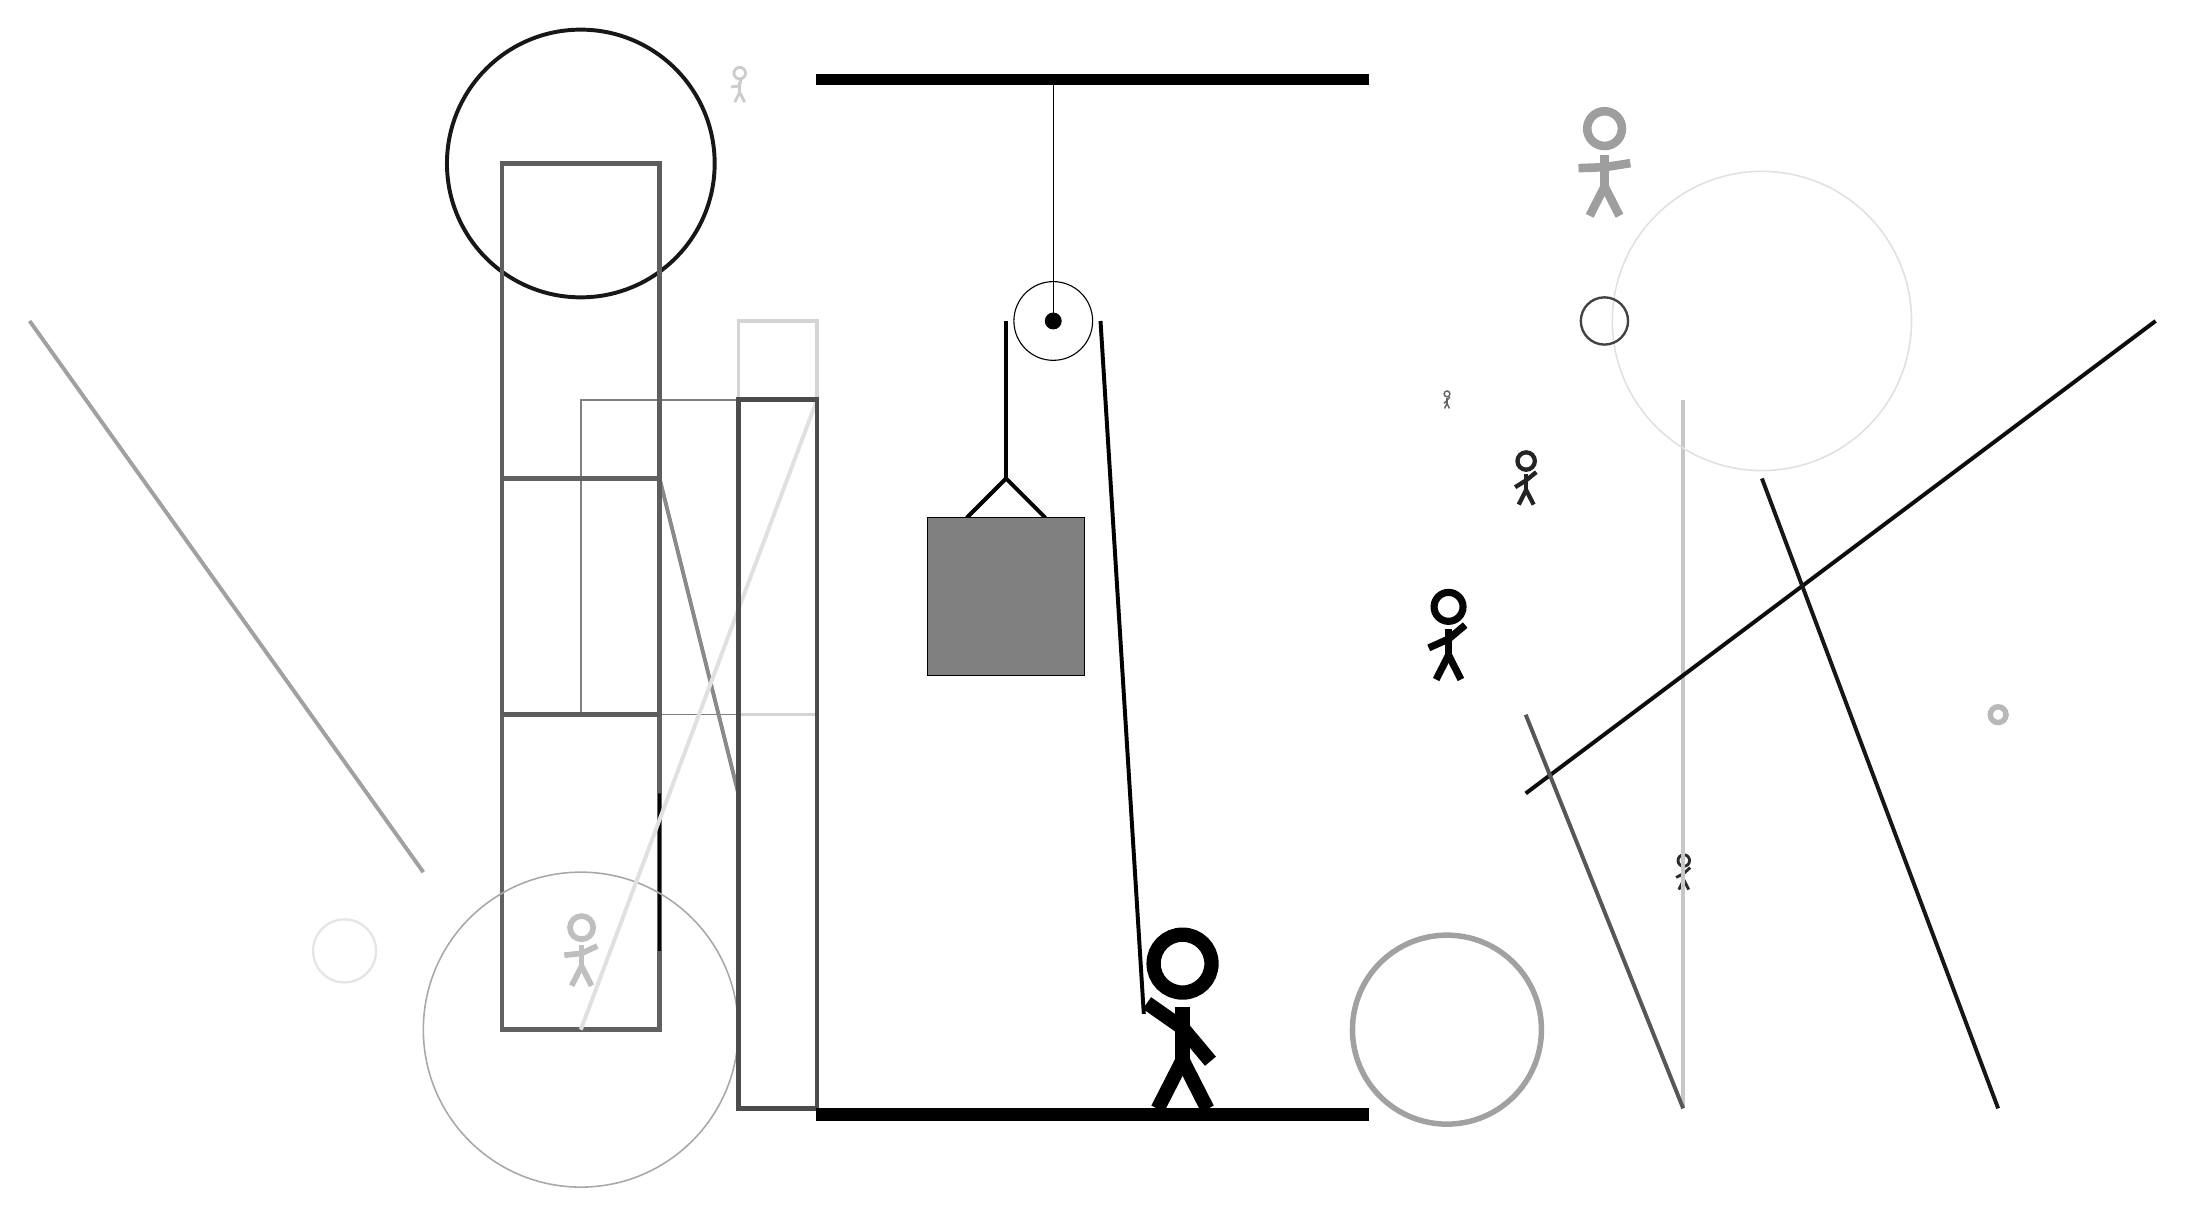
\begin{tikzpicture}
		%%%%% START %%%%%
		
		\draw[fill=black] (-2, 10) rectangle (5, 10.125);
		
		\draw (1, 7) circle (0.5);
		\draw[fill=black] (1, 7) circle (0.1);
		\draw (1, 10) -- (1, 7);
		
		\draw[line width=0.5mm] (-0.1, 4.5) -- (0.4, 5.0) -- (0.9, 4.5);
		\draw[fill=black!50] (-0.6, 4.5) rectangle (1.4, 2.5);
		
		\node[line width=0.5mm, color=black!25] at (-5, -1) {\Strichmaxerl[4][6][25]};
		
		\draw [line width=0.5mm, color=black!91](-5, 9) circle (1.7);
		\draw[line width=0.5mm, color=black!69](-2, -1) -- (-2, 3);
		\node[line width=0.4mm, color=black!83] at (9, 0) {\Strichmaxerl[2][28][42]};
		
		\draw[line width=0.2mm, color=black!50] (-3, 2) rectangle (-5, 6);
		\node[line width=0.4mm, color=black!61] at (6, 6) {\Strichmaxerl[1][46][50]};
		
		\draw[line width=0.6mm, color=black!62] (-4, 5) rectangle (-6, -2);
		
		\draw[line width=0.5mm, color=black!77](-2, 0) -- (-2, 3);
		\draw[line width=0.3mm, color=black!98] (-4, 1) rectangle (-4, -1);
		\node[line width=0.5mm, color=black!20] at (-3, 10) {\Strichmaxerl[2][6][81]};
		\draw[line width=0.5mm, color=black!46](-3, 1) -- (-4, 5);
		\draw[line width=0.4mm, color=black!17] (-2, 7) rectangle (-3, 2);
		\draw[line width=0.5mm, color=black!22](9, -3) -- (9, 6);
		
		\draw[line width=0.5mm, color=black!95](7, 1) -- (15, 7);
		\draw [line width=0.7mm, color=black!28](13, 2) circle (0.1);
		\draw [line width=0.4mm, color=black!66](7, 0) circle (0.0);
		\draw [line width=0.2mm, color=black!34](-5, -2) circle (2.0);
		
		\node[line width=0.2mm, color=black!86] at (7, 5) {\Strichmaxerl[3][32][39]};
		\draw [line width=0.7mm, color=black!37](6, -2) circle (1.2);
		
		\draw[line width=0.5mm, color=black!91](10, 5) -- (13, -3);
		\draw [line width=0.2mm, color=black!12](10, 7) circle (1.9);
		
		\node[line width=0.2mm, color=black!98] at (6, 3) {\Strichmaxerl[5][24][40]};
		\node[line width=0.2mm, color=black!38] at (8, 9) {\Strichmaxerl[6][2][9]};
		\draw [line width=0.3mm, color=black!10](-8, -1) circle (0.4);
		\draw [line width=0.3mm, color=black!74](8, 7) circle (0.3);
		\draw[line width=0.6mm, color=black!63] (-4, 9) rectangle (-6, 2);
		\draw[line width=0.5mm, color=black!12](-2, 6) -- (-5, -2);
		\draw[line width=0.5mm, color=black!66](7, 2) -- (9, -3);
		\draw[line width=0.5mm, color=black!37](-7, 0) -- (-12, 7);
		\draw[line width=0.6mm, color=black!70] (-3, -3) rectangle (-2, 6);
		
		\draw[line width=0.5mm] (0.4, 7) -- (0.4, 5.0);
		\centerarc[line width=0.5mm](1, 7)(0:180:0.6);
		\draw[line width=0.5mm](1.6, 7) -- (2.15, -1.8);
		
		\node at (2.6, -1.9) {\Strichmaxerl[10][-35][-50]};
		
		\draw[fill=black] (-2, -3) rectangle (5, -3.15);
		
		%%%%% END %%%%%
	\end{tikzpicture}
\end{document}